% Pooled group bids (analyze/pooled_analysis.py, plan "pooled").
\begin{figure}[H]
    \centering
    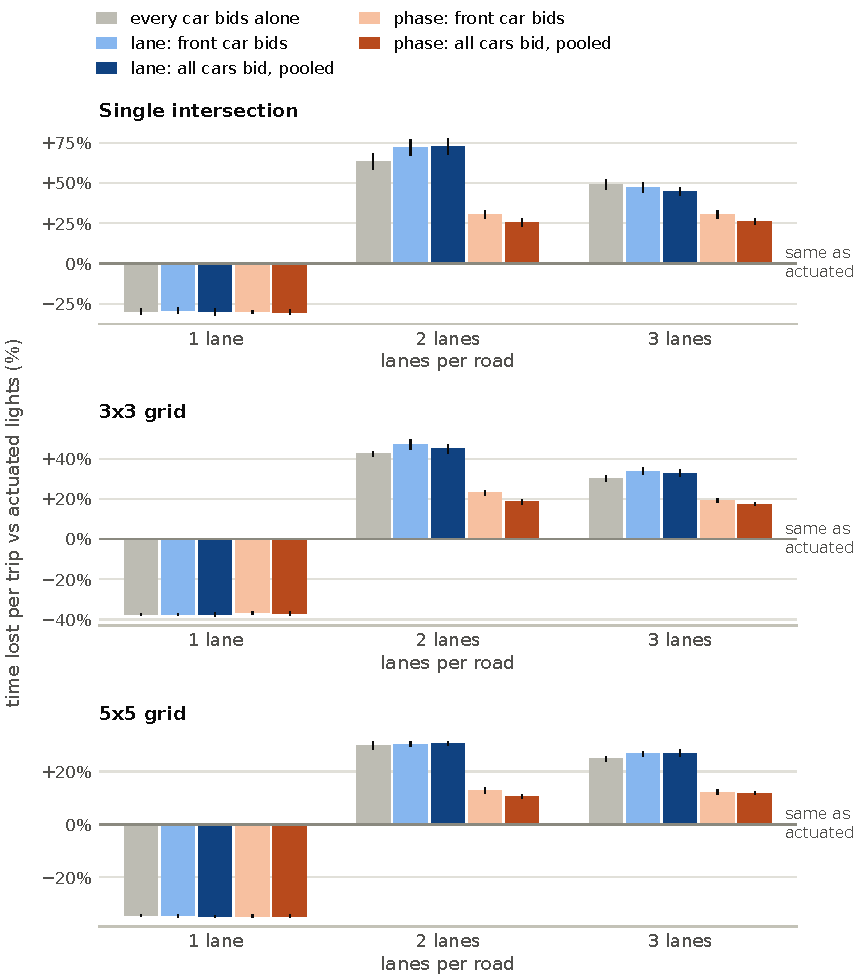
\includegraphics[width=\linewidth]{pooled_units.pdf}
    \caption{Time lost per trip under each bidding unit, compared with actuated lights (0\%) on
    the same trips, for the even mix of the five fixed rules. Every car bids alone; the front car
    of each lane or signal phase bids for it; or every car of the lane or phase bids from its own
    balance by its own rule and the bids are summed (pooled; each winning car pays its own bid
    when contested, and the payment is shared among the cars of the losing groups). Reference
    setting, 7 warm-up days, then the same 7-day evaluation week; bars are means of 10
    seeds, whiskers 95\% intervals; each panel has its own scale.}
    \label{fig:pooled_units}
\end{figure}

\begin{figure}[H]
    \centering
    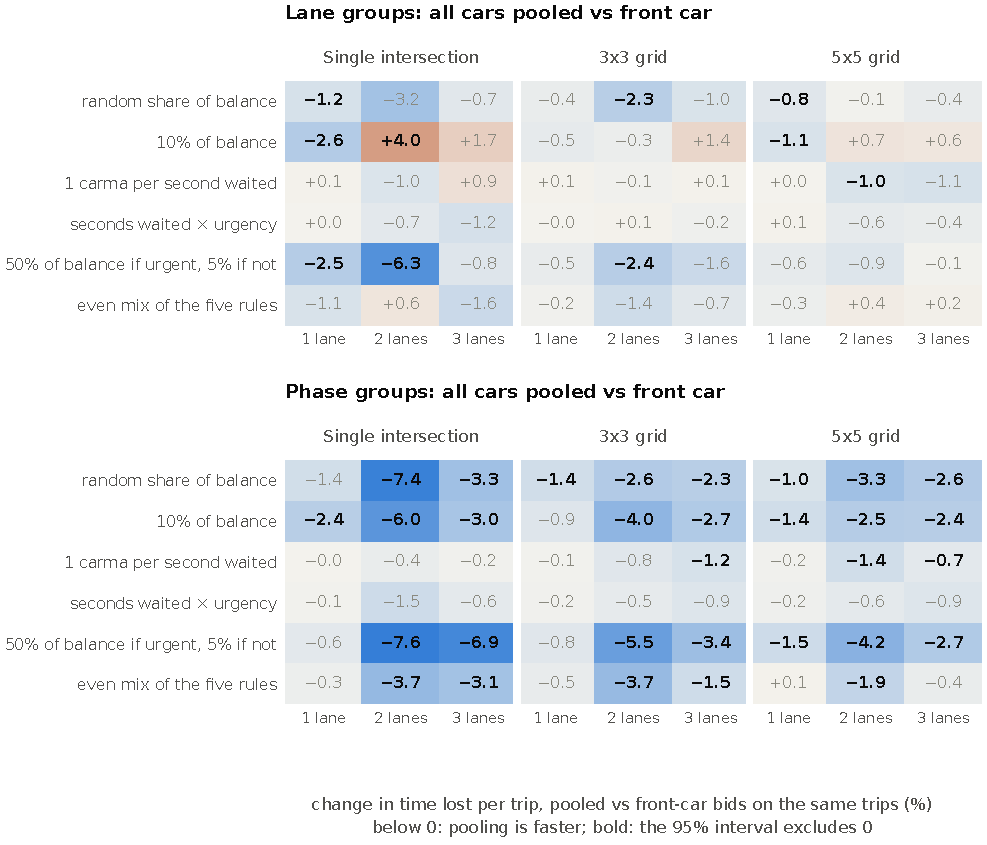
\includegraphics[width=\linewidth]{pooled_effect.pdf}
    \caption{What pooling changes, rule by rule: time lost per trip with every car of the group
    bidding (pooled) against only the front car bidding, same rule, trips and seed, as a
    percentage of the front-car time lost. Blue: pooling is faster. Bold: the 95\% interval over
    10 seeds excludes 0. Settings as in Figure~\ref{fig:pooled_units}.}
    \label{fig:pooled_effect}
\end{figure}
